\chapter{Heat MPI parallelization}

% exam: alternative for reduction code (assignment 5)

In this assignment, the heat application was parallelized using MPI. Only the data used by each process was initialized locally. This way, the Jacobi relaxation and coarsening for the output were parallelized. To split the domain, MPI Cartesian topology was used. 

Both blocking and non-blocking communication were trialed. Different ways of splitting up the domain were tried and compared, with divisions done in the x- and y-dimensions, and as a combination.

Figure \ref{fig:speedups-mpi-1d2d} shows the speedups for different processor configurations compared to the sequential version.

\begin{figure}[h]
    \centering
    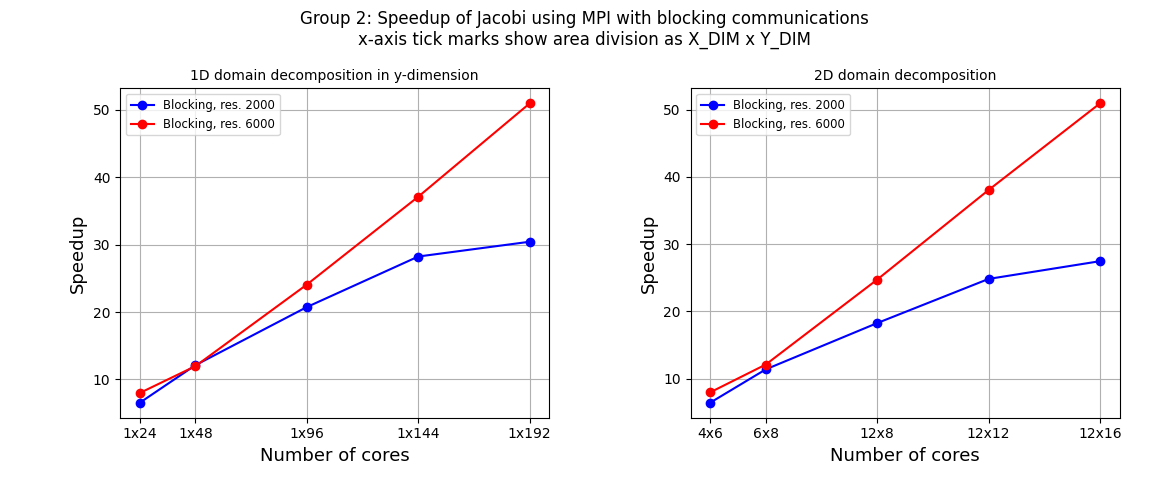
\includegraphics[scale=0.55]{figures/group2_jacobiMPI_1d_2d.png}
    \caption{Comparison of speedups for domain splitting in only the y-dimension, and in both dimensions.}
    \label{fig:speedups-mpi-1d2d}
\end{figure}

As can be seen from the results, for the maximum number of cores available, 192 cores spread over 4 nodes, the speedups achieved by the program are just above 50 for the higher resolution, and around 30 for the lower resolution. These results are worse than for the OpenMP parallelization, where 48 cores achieved a speedup of 27, compared to 13 for the MPI implementation. This is likely due to the increased communication overhead of MPI processes, and the fact that OpenMP threads could more effectively utilize the shared memory within one node.

It can also be seen that the there is a performance difference between the two resolutions, with the smaller resolution fairing worse. For the smaller resolution, communication between processes needs to happen more frequently as the relaxation computation is faster, which adds overhead. Additionally, the time spent for code startup is a larger percentage of the total execution time for the smaller resolution. These factors may explain the lower speedups of the 2000 resolution.

The figure also shows that splitting the domain in only one dimension made no significant difference to splitting it in two dimensions. This seems incorrect, as splitting the domain in both dimensions should provide a performance boost. This is because there are fewer border cells to be communicated between processes when the domain is split in two dimensions, requiring less communication overhead. The reason for these counter-intuitive results was not found, as the domain is split correctly by the program. One area that could be the cause is the communication of non-contiguous columns, as splitting the domain only in the x-dimension, causing only columns to be communicated, has a worse speedup when compared to splitting in only the y-dimension, where only contiguous rows are communicated. However, for now this is still unconfirmed as we could not find the fault in the code.

Blocking and non-blocking communications were compared, as implementing non-blocking communication can sometimes result in a performance boost due to communication latency being hidden by computationally heavy parts of the program. The inner part of the local Jacobi relaxation was computed while the communications were started. Then, MPI\_Waitall() was called to wait for the communications to finish. Figure \ref{fig:mpi-block_vs_nonblock} shows the results of the comparison. 

\begin{figure}[h]
    \centering
    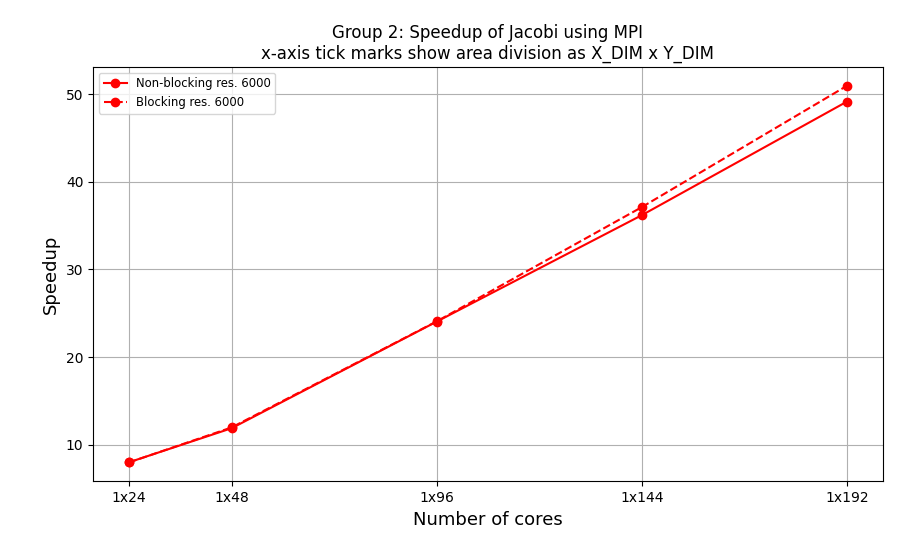
\includegraphics[scale=0.6]{figures/group2_jacobiMPI_blocking_nonblocking_6000.png}
    \caption{Comparison of non-blocking and blocking communication speedups for resolution 6000.}
    \label{fig:mpi-block_vs_nonblock}
\end{figure}

As can be seen from the figure, non-blocking communication did not yield a boost in performance, but slightly decreased it. As it is also more cumbersome for the programmer to implement, it is not worth the effort for this use case. The decrease in performance is likely due to the computation of the Jacobi relaxation in the inner domain not being heavy enough to hide the communication latency. Non-blocking communication also introduces additional overhead due to the use of MPI\_Requests. One way to improve the performance of non-blocking communication could be to only exchange data every N iterations, but this would make the parallel code incorrect when compared to the sequential code. 

Overall, this assignment showed that implementing MPI with blocking communication yields scalable results for parallelizing the Jacobi method.